\chapter{Results}

The aim of this project is to create a boundary representation of an indoor environment from laser scan data. This section builds on the literature review and Method and describes the process undertaken to get a B-rep model.\\
\\
The point clouds are processes through an command line program that takes in the point cloud name as a parameter, then saves the B-rep model as an obj file with the same name and same file location as the point cloud.

	\section{Segmentation}
		The segmentation of the point cloud is done with a built in region growing function from Point Cloud Library. A detailed description of the region growing and normal calculation process is given in Section \ref{segmentation-method}.
		
		\subsection{Normal Calculation}
		
		Before segmentation can take place normals need to be calculated for each point in the cloud. Normals are calculated using a Principal components analysis, with the neighbourhood around the point, $k$, set to the nearest 40 points. 
		
		40 was chosen because it gives the best results, higher and the gaps at the corners of the room start to become very big making segments smaller, as well as no co-planar features are detected for example a door will become part of the wall. Any smaller and there is too much variation in the normals making the region growing segmentation leave holes in the planar segments such as in Figure \ref{fig:k=5}:
		
		
		\begin{figure}[H]
			\centering
			\includegraphics[width=1\linewidth]{"Includes/images/Normal Comp/k = 5 ver 2"}
			\caption{$k$ = 5}
			\label{fig:k=5}
		\end{figure}
		
		\begin{figure}[H]
			\centering
			\includegraphics[width=1\linewidth]{"Includes/images/Normal Comp/k = 200 ver 2"}
			\caption{$k$ = 200}
			\label{fig:k=200}
		\end{figure}
		
		Both images are done with the region growing parameters chosen in section \ref{RegionGrowParams}

		
		There is also a speed aspect to the neighbourhood size, smaller results in a much faster computation, and larger much slower. This is not a huge issue as the normal estimation function has multi-threading making it only take up to 10s at most. This is only about 5\% of the total run-time.
		
		
		\subsection{Region Growing}
		\label{RegionGrowParams}
			
		Once the normals have been calculated the point cloud is segmented using region growing. Region growing takes in 5 parameters; Minimum cluster size, Maximum cluster size,Search Method, Number of neighbours, Smoothness threshold and Curvature threshold.
		
		In the case of this project bigger segments are good, so the Maximum cluster size value was never set allowing clusters be as large as the need to be.
		
		The minimum cluster size was set to 5000 points because the chances of a significant wall section being less than 5000 points is very low, having this large number also removes a lot of the clutter in a room. Removing clutter is an important part of this project as any small segment thats not a part of the extent of the room (i.e. walls, roof or floor) will create problems with the rest of the program.
		
		
		\begin{figure}[H]
			\centering
			\includegraphics[width=1\linewidth]{"Includes/images/RegionGrowing/min-size = 100"}
			\caption{Minimum Cluster Size = 100}
			\label{fig:min-size=100}
		\end{figure}
		
		\begin{figure}[H]
			\centering
			\includegraphics[width=1\linewidth]{"Includes/images/RegionGrowing/min-size = 5000"}
			\caption{Minimum Cluster Size = 5000}
			\label{fig:min-size=5000}
		\end{figure}
		
		The Smoothness and Curvature thresholds are very important in this project as the outcome relies on planar segments so strict thresholds on curvature and smoothness are important to make sure that any segment is a planar segment and does not cover two sides of a room. You can see in Figure \ref{fig:NoSmoothCurv} that the roof and right hand wall are one segment, resulting in a fitted plane that goes at a 45\textdegree\: angle through the room. As well as the person in the figure who is large enough to pass all the tests but is most defiantly not a wall.
		
		
		\begin{figure}[H]
			\centering
			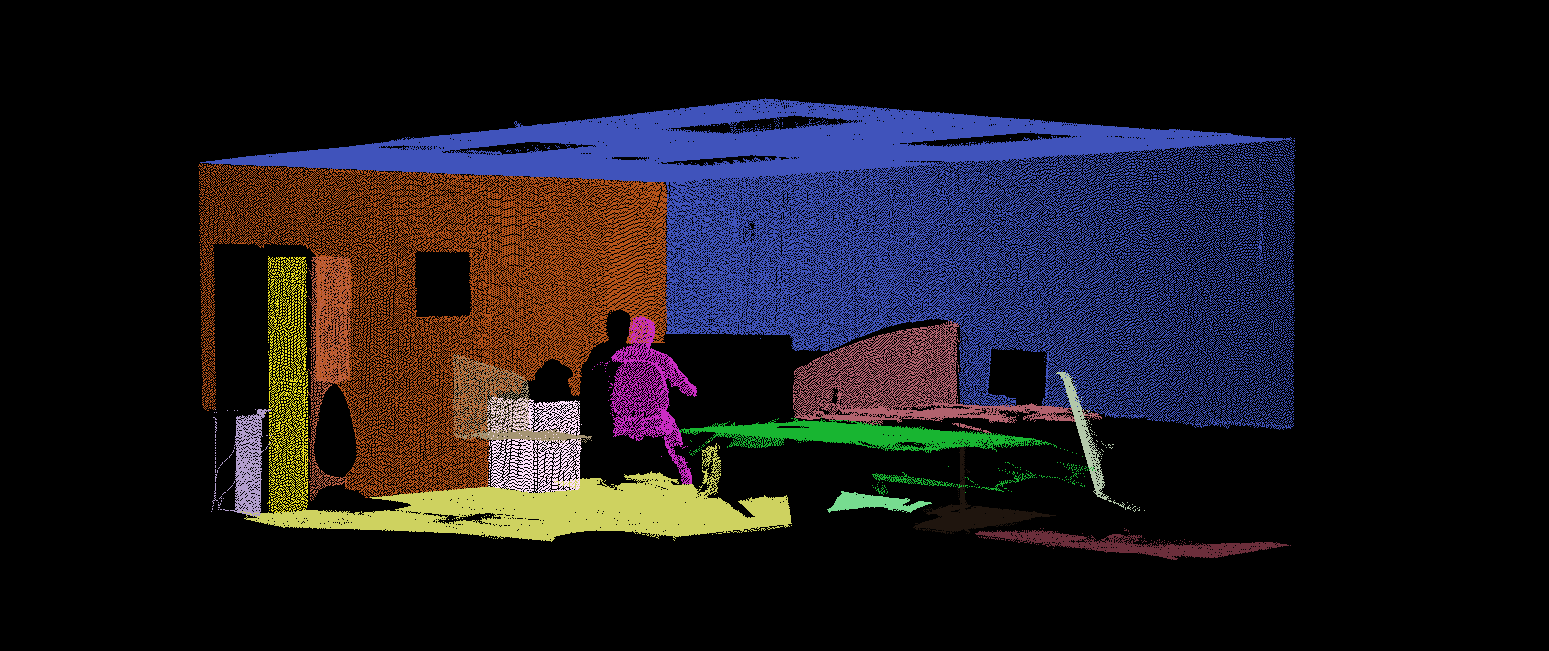
\includegraphics[width=1\linewidth]{Includes/images/RegionGrowing/NoSmoothCurv}
			\caption{Region Growing Run with no Smoothness or Curvature Thresholds set}
			\label{fig:NoSmoothCurv}
		\end{figure}
	
		Number of neighbours makes the door show up!
		
		
\begin{figure}[H]
\centering
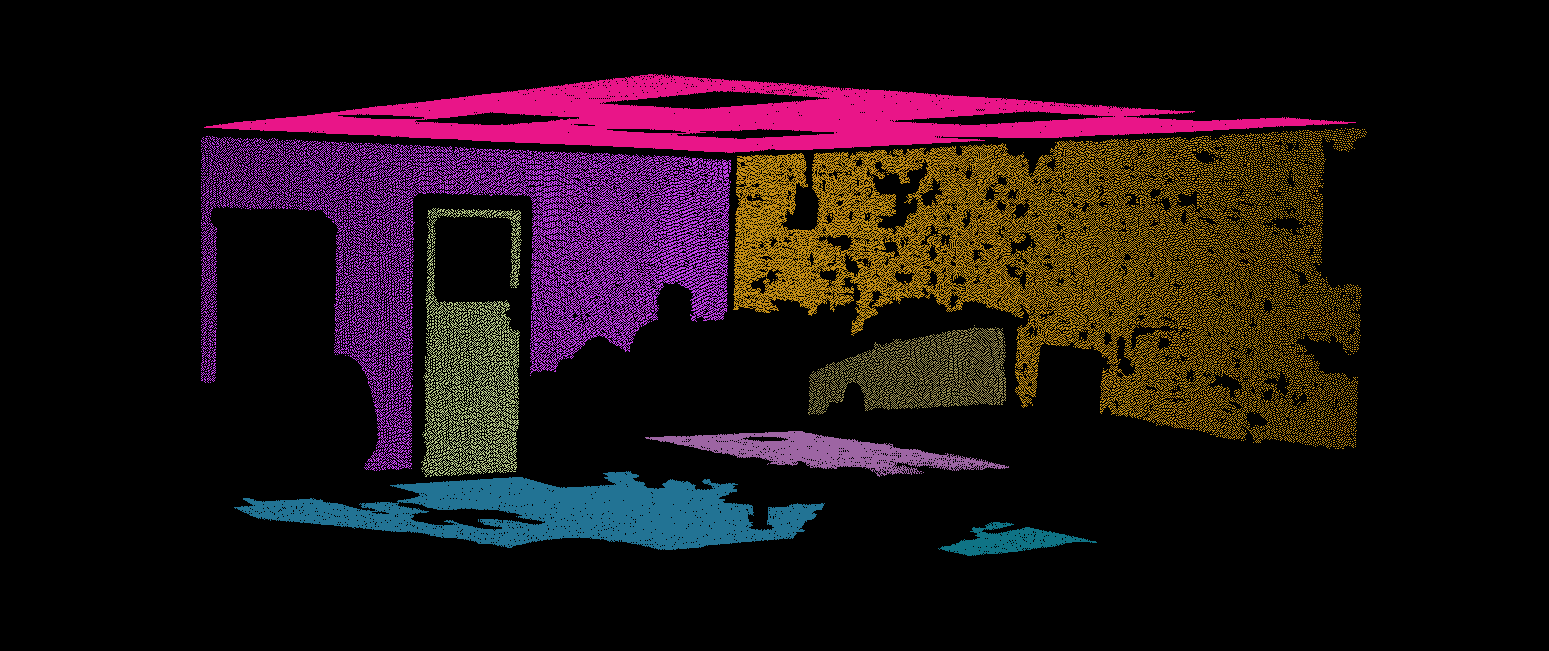
\includegraphics[width=1\linewidth]{Includes/images/RegionGrowing/neighbours-5}
\caption{}
\label{fig:neighbours-5}
\end{figure}

\begin{figure}[H]
\centering
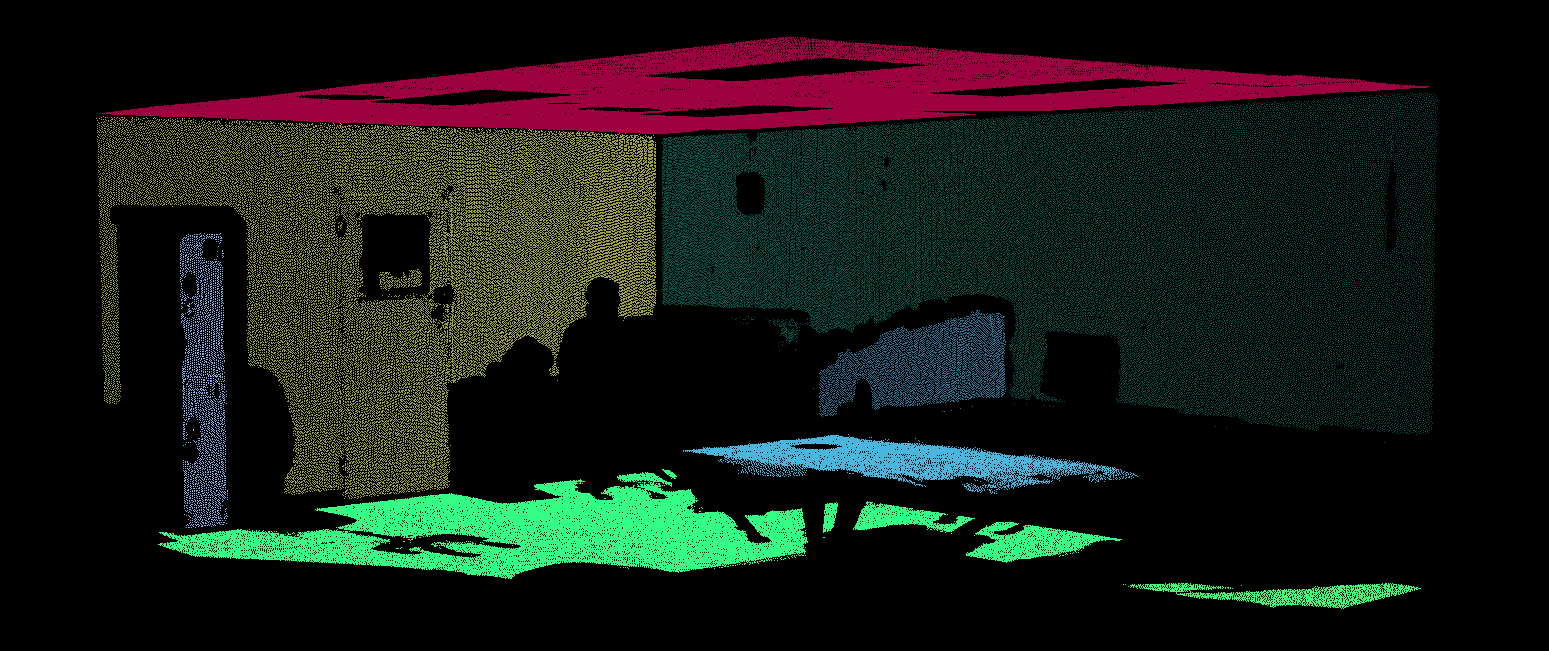
\includegraphics[width=1\linewidth]{Includes/images/RegionGrowing/neighbours-200}
\caption{}
\label{fig:neighbours-200}
\end{figure}

		
		\begin{lstlisting}
MinClusterSize = 5000;
NumberOfNeighbours = 20;
SmoothnessThreshold = (1.0 * M_PI / 180);
CurvatureThreshold = 1.0;
		\end{lstlisting}
		
		
	
			The segmentation of the point cloud is the most time consuming function in the whole process, taking up on average 80\% of total run-time.
			
			Once again the speed of the process depends greatly on the parameters set
		
		

	\section{Surface Extraction}
	
	It is immediately evident in Figure \ref{fig:RG-noUnclass} that there are too many small segments that are not necessary and irreverent to the final output. So it becomes necessary to filter these segments out.
	
	To begin this, a vector of the segments is created after the region growing has taken place.


	\subsection{Segment selection}
		The vector of segments created in the segmentation section of the program is not entirely useful due to the fact that it contains segments all the segments.
		
		Most of the segments are small cluttering objects, like sides of desks of tops of tables. In process of trying to extract the boundaries of a room all this clutter is unnecessary, so we need to filter it out somehow.
		\subsubsection{filtering out Horizontal and Vertical surfaces}
			To start this process, the vector of segments is split up into two separate vectors, horizontal segments and vertical segments. This is done by iterating through the segments and deciding which category they fall under.
			
			By fitting a plane to the segment using the RANSAC method outlined above we can determine its orientation from the coefficients $a$, $b$, and $c$ of the planes equation.
			
			\begin{equation}
			ax + by + cz = d  \quad\quad
			\vec{n}_{segment} = \begin{bmatrix}a\\b\\c\end{bmatrix}
			\end{equation}
			
			So with the normal of the segment determined we can compare it to a vector that runs parallel to the Z axis. The obvious choice of a vertical vector is:
			
			\begin{equation}
			\vec{v} = \begin{bmatrix}0\\0\\1\end{bmatrix}
			\end{equation}
			
			Then to get the angle between the two vectors we take the dot product:
			
			\begin{equation}
			\vec{n}_{segment}\cdot \vec{v} = \norm{\vec{n}_{segment}} \norm{\vec{v}} cos \theta
			\end{equation}
			
			Solving for $\theta$ gives us the angle between the segment and vertical. From here it is easy to decide if a segment is horizontal or vertical, by seeing if $\theta$ is closer to 0\textdegree/180\textdegree or 90\textdegree.
			
		\subsubsection{Selection of Vertical Segments}
			
			The vertical extent of the segment is determined by finding the highest and lowest points and getting the distance between them:
			
			\begin{equation}
			Vertical \: Extent = \sqrt{(x_{max} - x_{min})^2+(y_{max} - y_{min})^2+(z_{max} - z_{min})^2}
			\end{equation}
			
			If the vertical extent of a segment is less that 1m, it is safe to assume that the segment does not make up part of the walls of the room.\\
			\\
			The process of finding the highest and lowest points in a segment is simply a loop through all the points keeping the points with the highest and lowest z values.\\
			\\
			The selection based on Angle is simply an extension of the previous method for splitting the the segments based on orientation, but with a much more strict angle defining vertical, $\theta$ must fall within $\pm$10\textdegree of 90\textdegree:
			
			\begin{equation}
			80\textdegree < \theta < 100\textdegree
			\end{equation}

			
	\section{Model Generation}
	
	
	\section{Creating Obj file}
			
					
